\begin{equation}
    \begin{gathered}
        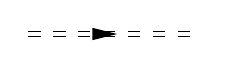
\begin{tikzpicture}[x=0.75pt,y=0.75pt,yscale=-1,xscale=1]
            %uncomment if require: \path (0,300); %set diagram left start at 0, and has height of 300
            
            %Straight Lines [id:da2580381812771073] 
            \draw  [dash pattern={on 4.5pt off 4.5pt}]  (167.71,167.57) -- (249.41,167.57) ;
            %Straight Lines [id:da1812296474143189] 
            \draw  [dash pattern={on 4.5pt off 4.5pt}]  (167.71,169.57) -- (249.41,169.57) ;
            %Straight Lines [id:da891236591561634] 
            \draw    (210.56,168.57) ;
            \draw [shift={(210.56,168.57)}, rotate = 180] [fill={rgb, 255:red, 0; green, 0; blue, 0 }  ][line width=0.08]  [draw opacity=0] (12,-3) -- (0,0) -- (12,3) -- cycle    ;
            \end{tikzpicture}
    \end{gathered} = \begin{gathered}
        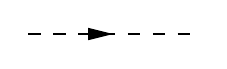
\begin{tikzpicture}[x=0.75pt,y=0.75pt,yscale=-1,xscale=1]
            %uncomment if require: \path (0,300); %set diagram left start at 0, and has height of 300
            
            %Straight Lines [id:da2580381812771073] 
            \draw  [dash pattern={on 4.5pt off 4.5pt}]  (167.71,167.57) -- (249.41,167.57) ;
            \draw [shift={(208.56,167.57)}, rotate = 180] [fill={rgb, 255:red, 0; green, 0; blue, 0 }  ][line width=0.08]  [draw opacity=0] (12,-3) -- (0,0) -- (12,3) -- cycle    ;
            \end{tikzpicture}
    \end{gathered} + \begin{gathered}
        \begin{tikzpicture}[x=0.75pt,y=0.75pt,yscale=-1,xscale=1]
            %uncomment if require: \path (0,300); %set diagram left start at 0, and has height of 300
            
            %Straight Lines [id:da24576617158021508] 
            \draw  [dash pattern={on 4.5pt off 4.5pt}]  (100,125) -- (165.71,125) ;
            \draw [shift={(132.85,125)}, rotate = 180] [fill={rgb, 255:red, 0; green, 0; blue, 0 }  ][line width=0.08]  [draw opacity=0] (12,-3) -- (0,0) -- (12,3) -- cycle    ;
            %Shape: Circle [id:dp6762265906581268] 
            \draw   (165.71,125) .. controls (165.71,108.1) and (179.41,94.4) .. (196.31,94.4) .. controls (213.21,94.4) and (226.91,108.1) .. (226.91,125) .. controls (226.91,141.9) and (213.21,155.6) .. (196.31,155.6) .. controls (179.41,155.6) and (165.71,141.9) .. (165.71,125) -- cycle ;
            %Straight Lines [id:da46135211886694005] 
            \draw  [dash pattern={on 4.5pt off 4.5pt}]  (226.91,125) -- (292.62,125) ;
            \draw [shift={(259.76,125)}, rotate = 180] [fill={rgb, 255:red, 0; green, 0; blue, 0 }  ][line width=0.08]  [draw opacity=0] (12,-3) -- (0,0) -- (12,3) -- cycle    ;
            %Straight Lines [id:da09338269031575619] 
            \draw    (203.31,94.4) ;
            \draw [shift={(203.31,94.4)}, rotate = 180] [fill={rgb, 255:red, 0; green, 0; blue, 0 }  ][line width=0.08]  [draw opacity=0] (12,-3) -- (0,0) -- (12,3) -- cycle    ;
            %Straight Lines [id:da4104133236840597] 
            \draw    (203.31,154.6) ;
            \draw [shift={(203.31,154.6)}, rotate = 180] [fill={rgb, 255:red, 0; green, 0; blue, 0 }  ][line width=0.08]  [draw opacity=0] (12,-3) -- (0,0) -- (12,3) -- cycle    ;
            \end{tikzpicture}                  
    \end{gathered},
    \label{eq:bcs-cooper-2nd-propagator}
\end{equation}